%
% test_report_v05.tex
%
% Copyright (C) 2021 by SpaceLab.
%
% OBDH 2.0 Documentation
%
% This work is licensed under the Creative Commons Attribution-ShareAlike 4.0
% International License. To view a copy of this license,
% visit http://creativecommons.org/licenses/by-sa/4.0/.
%

%
% \brief Test report of the v0.5 hardware.
%
% \author Gabriel Mariano Marcelino <gabriel.mm8@gmail.com>
%
% \institution Universidade Federal de Santa Catarina (UFSC)
%
% \version 0.6.0
%
% \date 2021/04/17
%

\chapter{Test Report of v0.5 Version} \label{anx:test-report-v05}

This appendix is a test report of the first manufactured and assembled PCB (version v0.5).

\begin{itemize}
    \item \textbf{PCB manufacturer}: PCBWay (China)
    \item \textbf{PCB assembly}: PCBWay (China)
    \item \textbf{PCB arrival date}: 2021/04/14
    \item \textbf{Execution date}: 2021/04/16 to \textcolor{red}{TBC}
    \item \textbf{Tester}: G. M. Marcelino
\end{itemize}

\section{Visual Inspection}

\begin{itemize}
    \item \textbf{Test description/Objective}: Inspection of the board, visually and with a multimeter, searching for fabrication and assembly failures.
    \item \textbf{Material}:
        \begin{itemize}
            \item Multimeter UNI-T DT830B
        \end{itemize}
    \item \textbf{Results}: The results of this test can be seen in Figures \ref{fig:obdh2-v05-top} (top view of the board) and \ref{fig:obdh2-v05-bottom} (bottom view of the board).
    \item \textbf{Conclusion}: No problems were identified on this test.
\end{itemize}

\begin{figure}[!ht]
    \begin{center}
        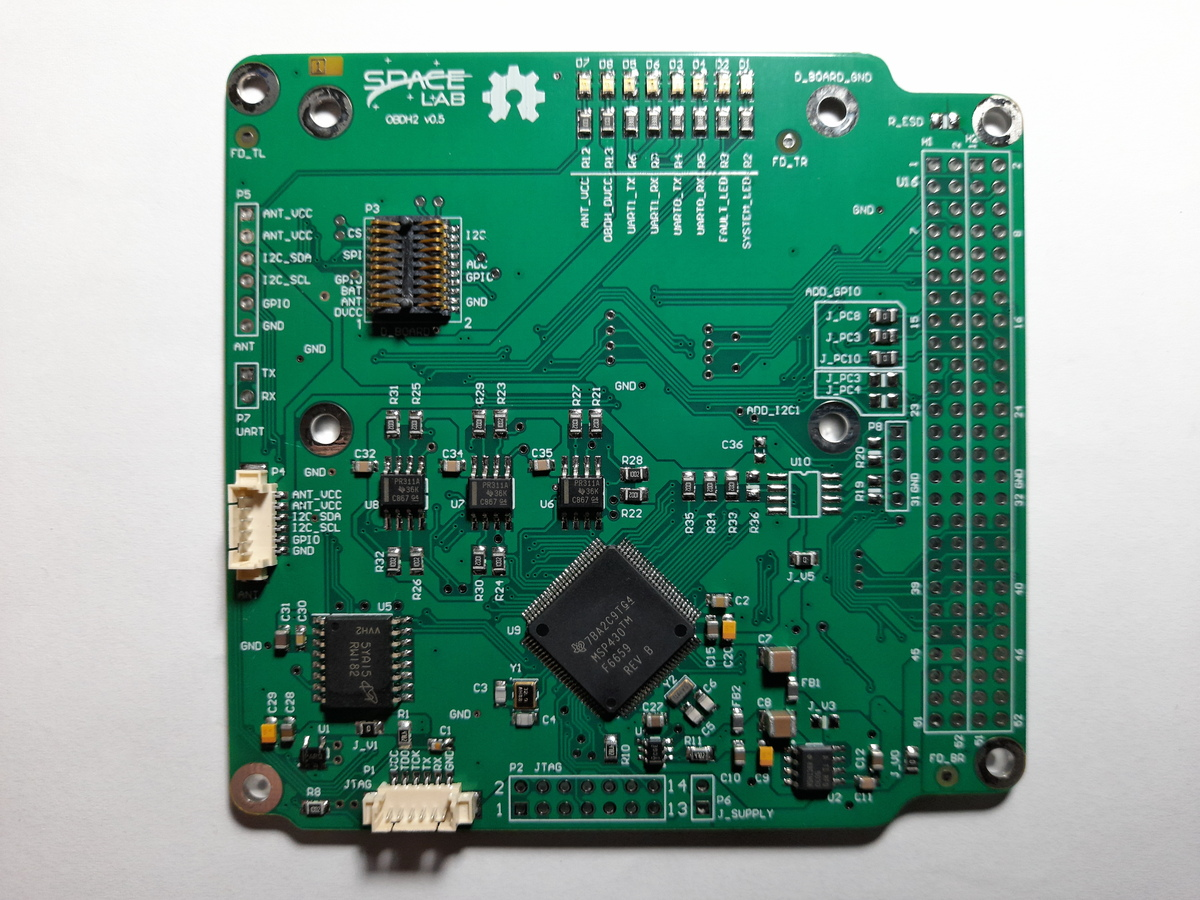
\includegraphics[width=\columnwidth]{figures/v05/obdh2-v05-top.jpg}
        \caption{Top view of the OBDH 2.0 v0.5 board.}
        \label{fig:obdh2-v05-top}
    \end{center}
\end{figure}

\begin{figure}[!ht]
    \begin{center}
        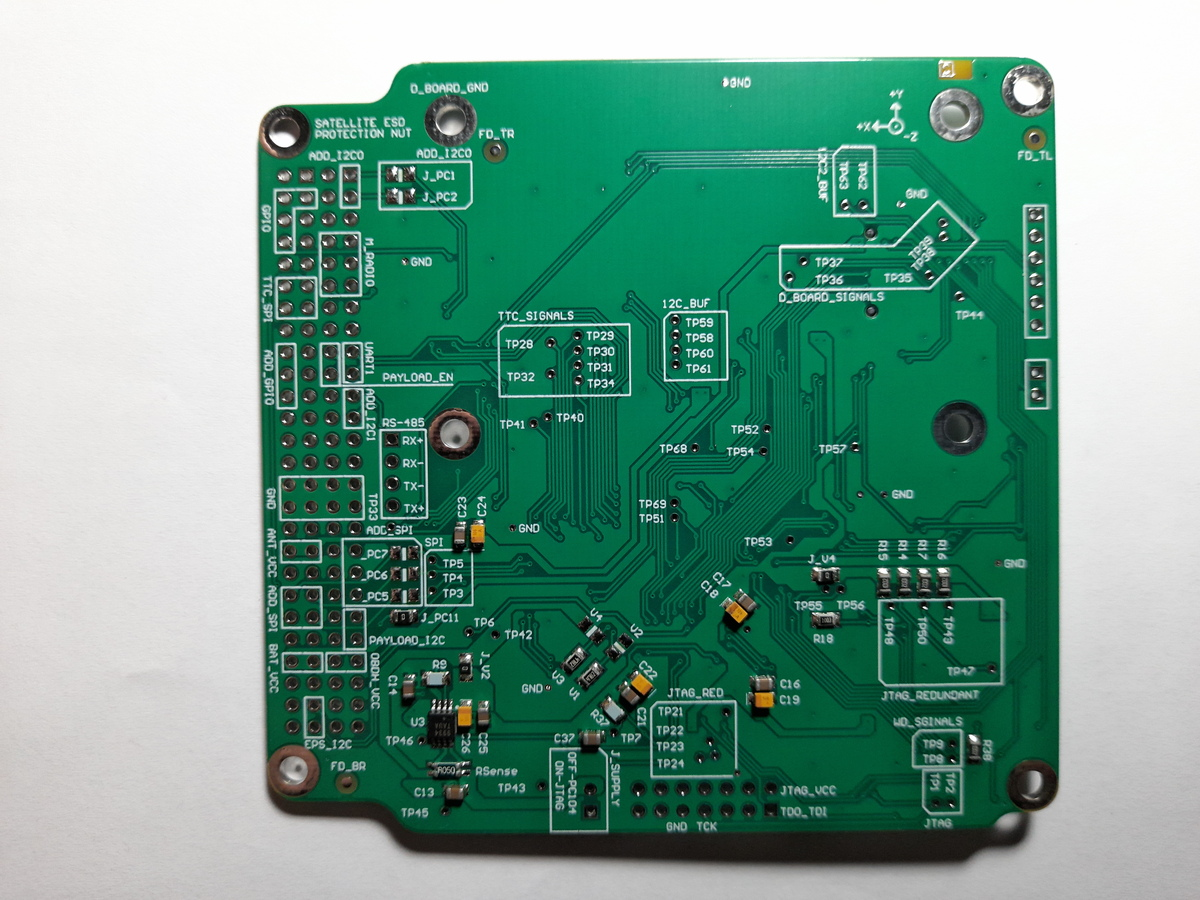
\includegraphics[width=\columnwidth]{figures/v05/obdh2-v05-bottom.jpg}
        \caption{Bottom view of the OBDH 2.0 v0.5 board.}
        \label{fig:obdh2-v05-bottom}
    \end{center}
\end{figure}

\section{Firmware Programming}

\begin{itemize}
    \item \textbf{Test description/Objective}: Inspection of the board, visually and with a multimeter, searching for fabrication and assembly mistakes.
    \item \textbf{Material}:
        \begin{itemize}
            \item Code Composer Studio v9.3.0
            \item MSP-FET Flash Emulation Tool
            \item USB-UART converter
            \item Screen (Linux software)
        \end{itemize}
    \item \textbf{Results}: The results of this are available in \autoref{fig:log-first-boot}, where the log messages of the first boot of the board can be seen.
    \item \textbf{Conclusion}: No problems were identified on this test.
\end{itemize}

\begin{figure}[!ht]
    \begin{center}
        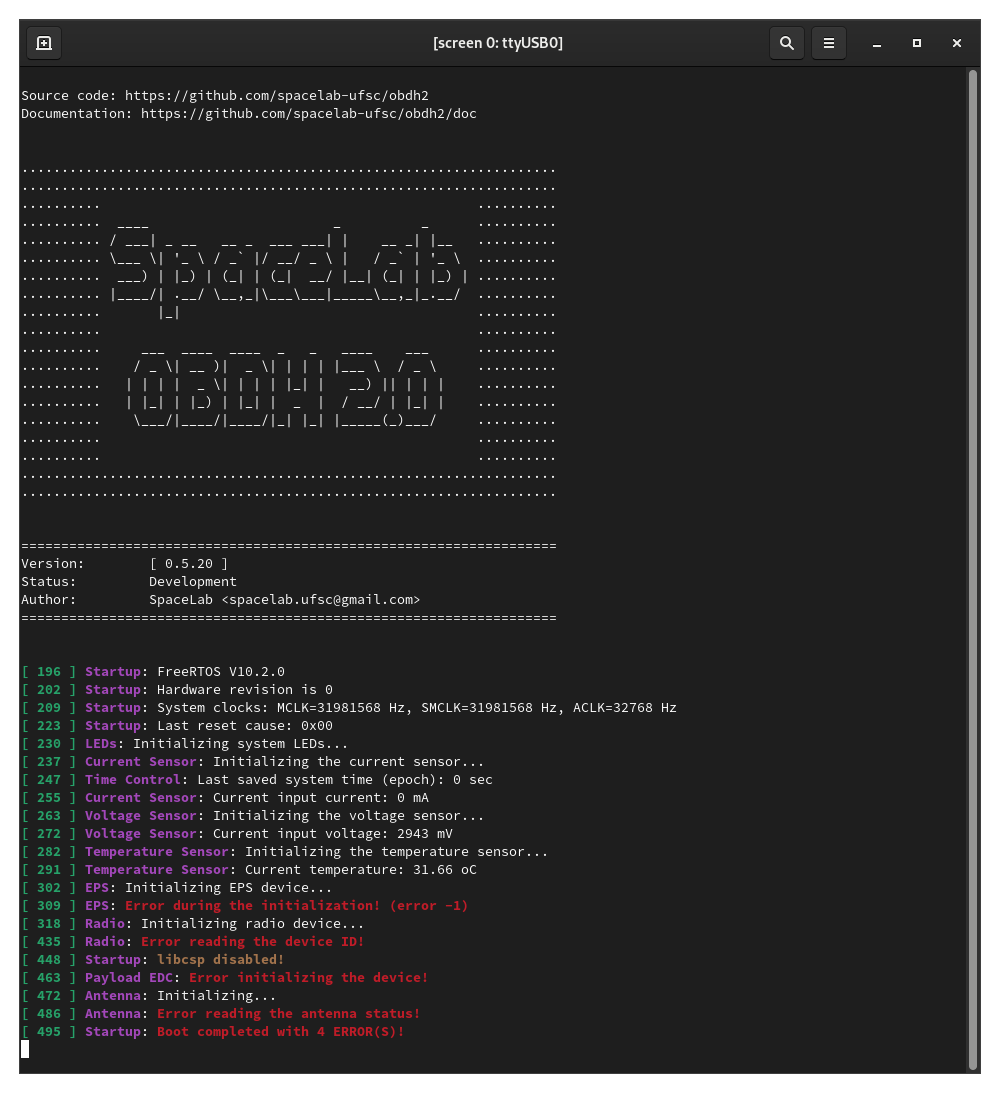
\includegraphics[width=0.7\columnwidth]{figures/v05/log-first-boot.png}
        \caption{Log messages during the first boot.}
        \label{fig:log-first-boot}
    \end{center}
\end{figure}

\section{Communication Busses}

\begin{itemize}
    \item \textbf{Test description/Objective}: Test the communication busses of the board, as listed below:
        \begin{itemize}
            \item I$^{2}$C Port 0
            \item I$^{2}$C Port 1
            \item I$^{2}$C Port 2
        \end{itemize}
    \item \textbf{Material}:
        \begin{itemize}
            \item Saleae Logic Analyzer (24 MHz, 8 channels)
            \item Saleae Logic software (v1.2.18)
            \item MSP-FET Flash Emulation Tool
        \end{itemize}
    \item \textbf{Results}: The results of this test can be seen in Figures \ref{fig:test-i2c-0}, \ref{fig:test-i2c-1} and \ref{fig:test-i2c-2}.
    \item \textbf{Conclusion:} No problems were identified on this test, all buses are working as expected.
\end{itemize}

\begin{figure}[!htb]
    \begin{center}
        \subfigure[Connections of the I$^{2}$C port 0 test.\label{fig:connections-i2c-0}]{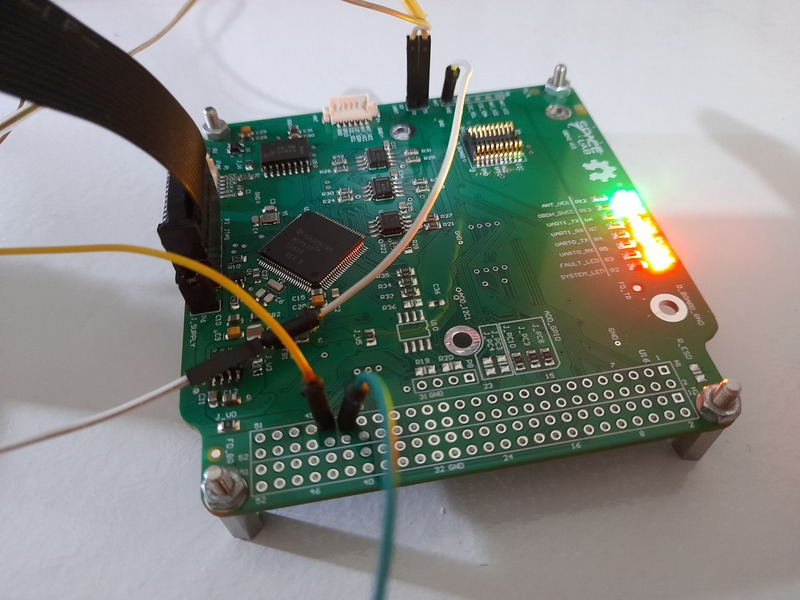
\includegraphics[height=0.22\textheight]{figures/v05/test-i2c-0.jpg}}
        ~
        \subfigure[Waveforms of the I$^{2}$C port 0 test.\label{fig:waveform-i2c-0}]{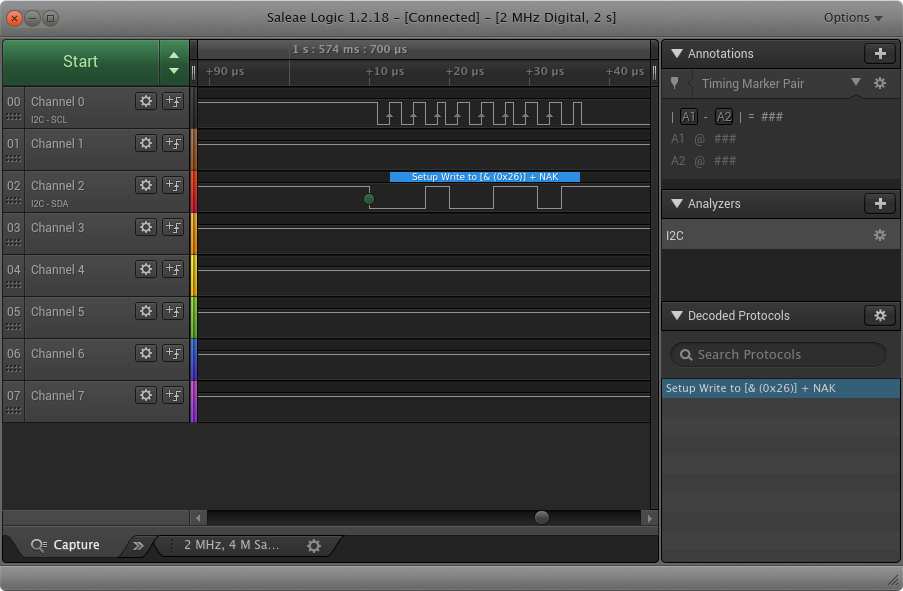
\includegraphics[height=0.22\textheight]{figures/v05/waveform-i2c-0.png}}
        \caption{I$^{2}$C port 0 test.}
        \label{fig:test-i2c-0}
    \end{center}
\end{figure}

%\begin{figure}[!ht]
%    \begin{center}
%        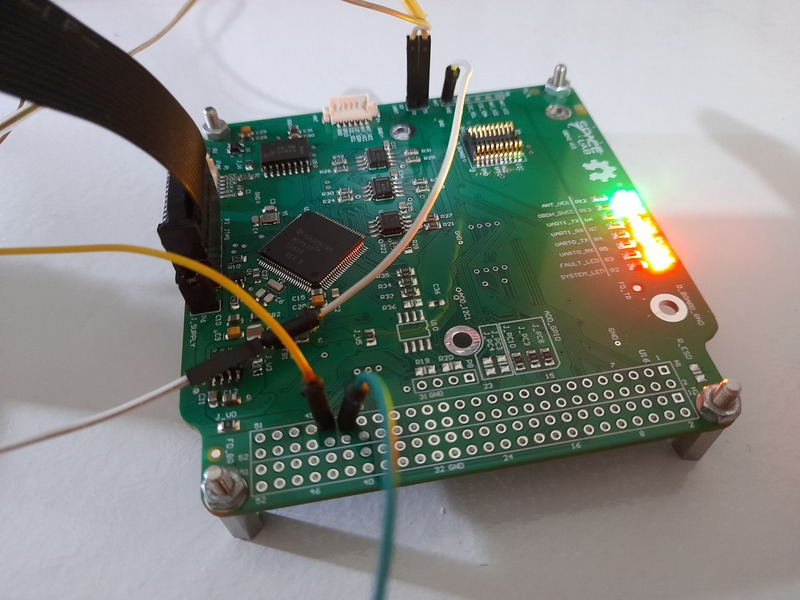
\includegraphics[width=0.7\columnwidth]{figures/v05/test-i2c-0.jpg}
%        \caption{Connections of the I2C port 0 test.}
%        \label{fig:test-i2c-0}
%    \end{center}
%\end{figure}
%
%\begin{figure}[!ht]
%    \begin{center}
%        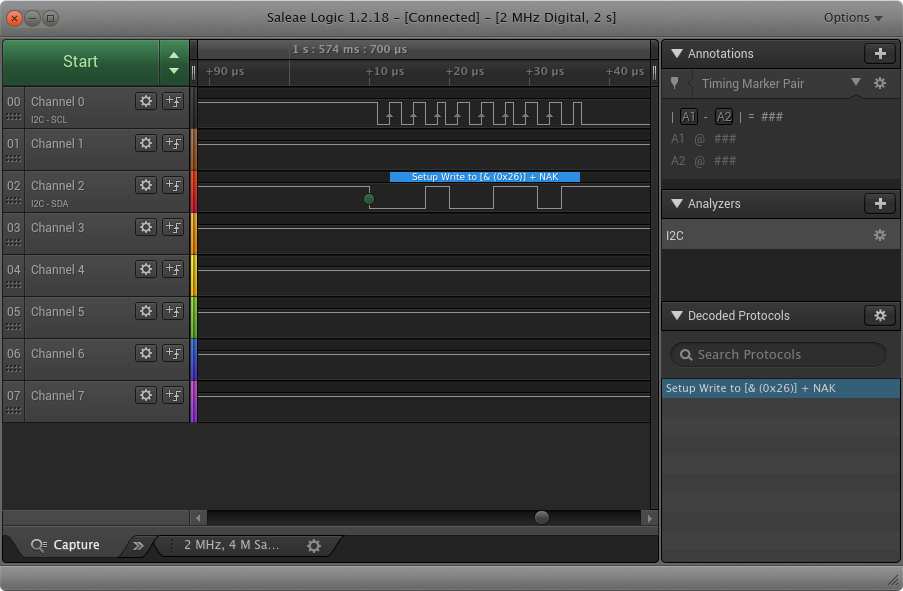
\includegraphics[width=\columnwidth]{figures/v05/waveform-i2c-0.png}
%        \caption{Waveform of the I2C port 0.}
%        \label{fig:waveform-i2c-0}
%    \end{center}
%\end{figure}

\begin{figure}[!htb]
    \begin{center}
        \subfigure[Connections of the I$^{2}$C port 1 test.\label{fig:connections-i2c-1}]{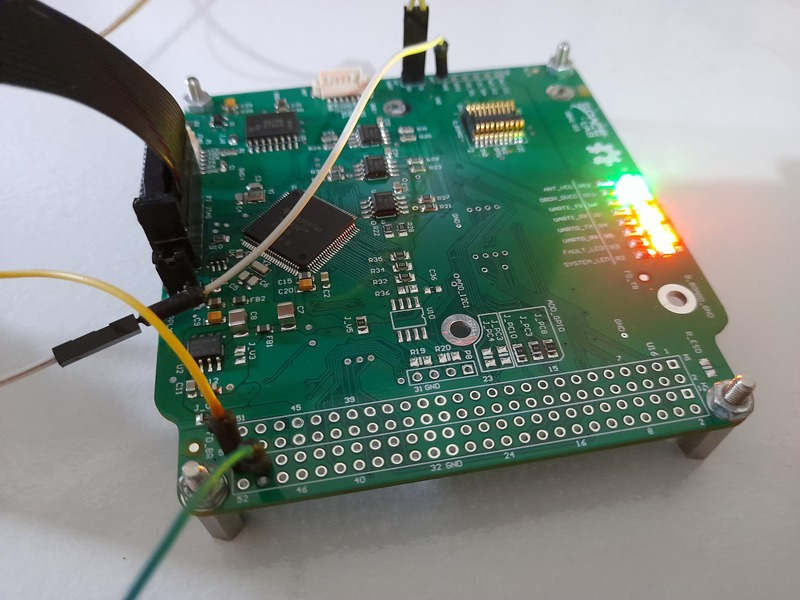
\includegraphics[height=0.22\textheight]{figures/v05/test-i2c-1.jpg}}
        ~
        \subfigure[Waveforms of the I$^{2}$C port 1 test.\label{fig:waveform-i2c-1}]{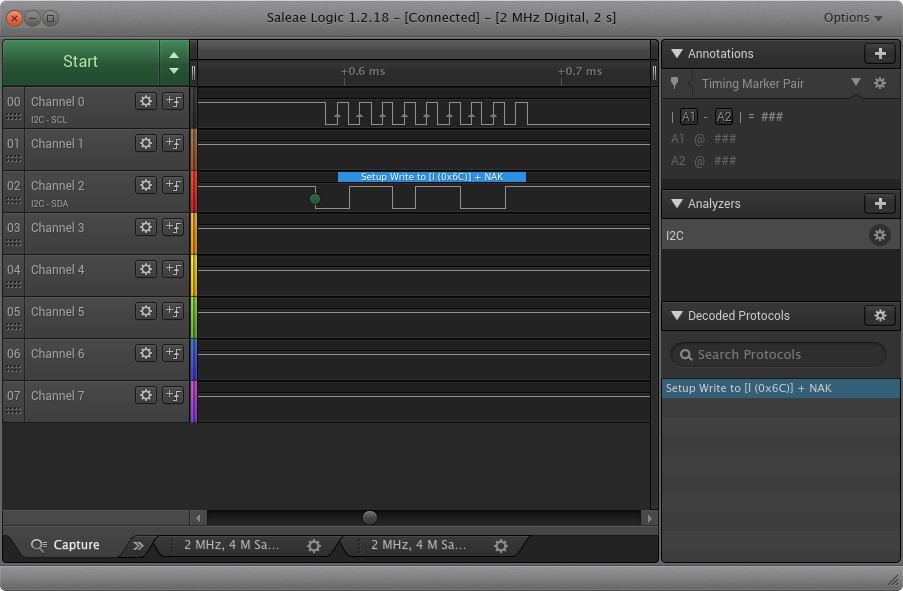
\includegraphics[height=0.22\textheight]{figures/v05/waveform-i2c-1.png}}
        \caption{I$^{2}$C port 1 test.}
        \label{fig:test-i2c-1}
    \end{center}
\end{figure}

%\begin{figure}[!ht]
%    \begin{center}
%        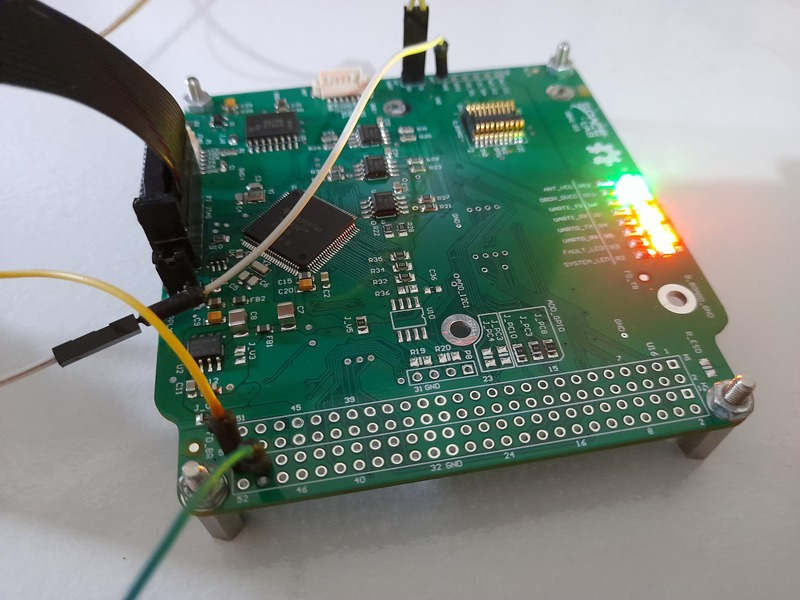
\includegraphics[width=0.7\columnwidth]{figures/v05/test-i2c-1.jpg}
%        \caption{Connections of the I2C port 1 test.}
%        \label{fig:test-i2c-1}
%    \end{center}
%\end{figure}
%
%\begin{figure}[!ht]
%    \begin{center}
%        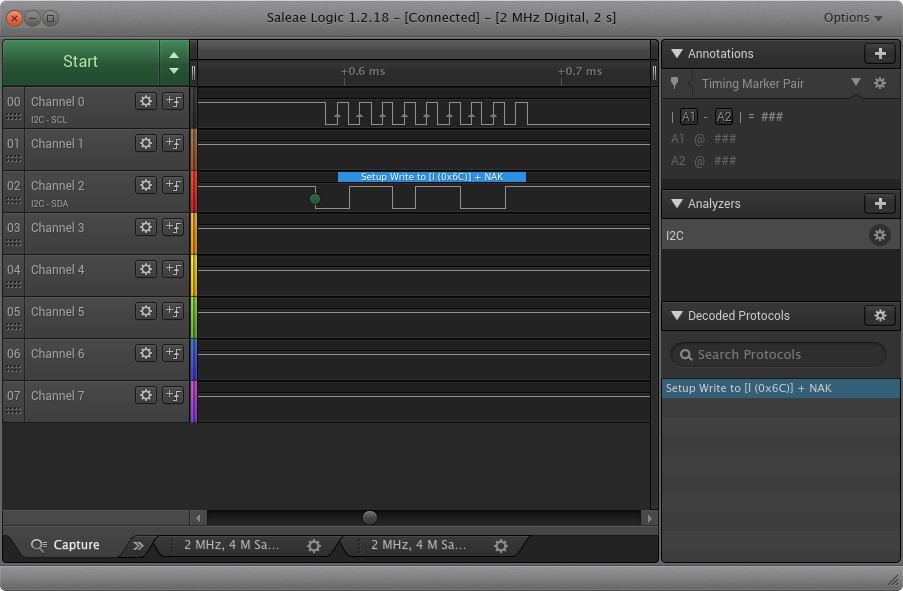
\includegraphics[width=\columnwidth]{figures/v05/waveform-i2c-1.png}
%        \caption{Waveform of the I2C port 1.}
%        \label{fig:waveform-i2c-1}
%    \end{center}
%\end{figure}

\begin{figure}[!htb]
    \begin{center}
        \subfigure[Connections of the I$^{2}$C port 2 test.\label{fig:connections-i2c-2}]{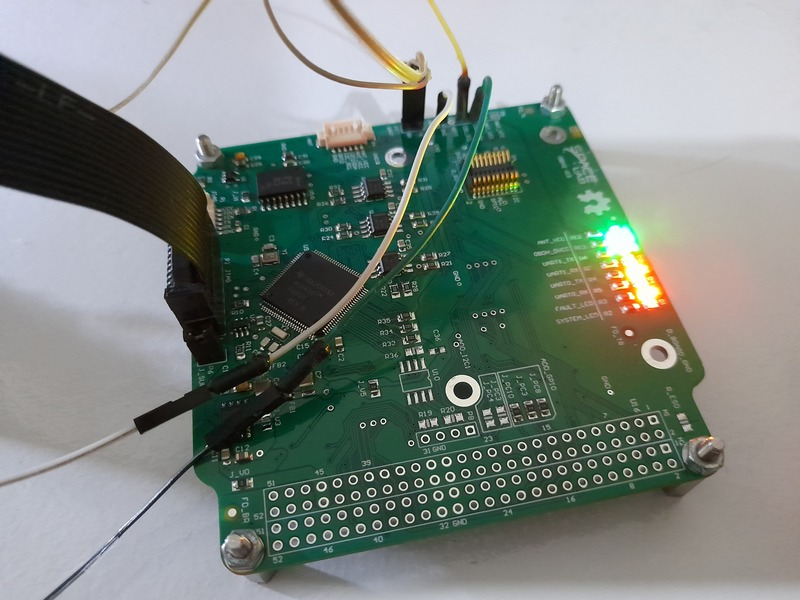
\includegraphics[height=0.22\textheight]{figures/v05/test-i2c-2.jpg}}
        ~
        \subfigure[Waveforms of the I$^{2}$C port 2 test.\label{fig:waveform-i2c-2}]{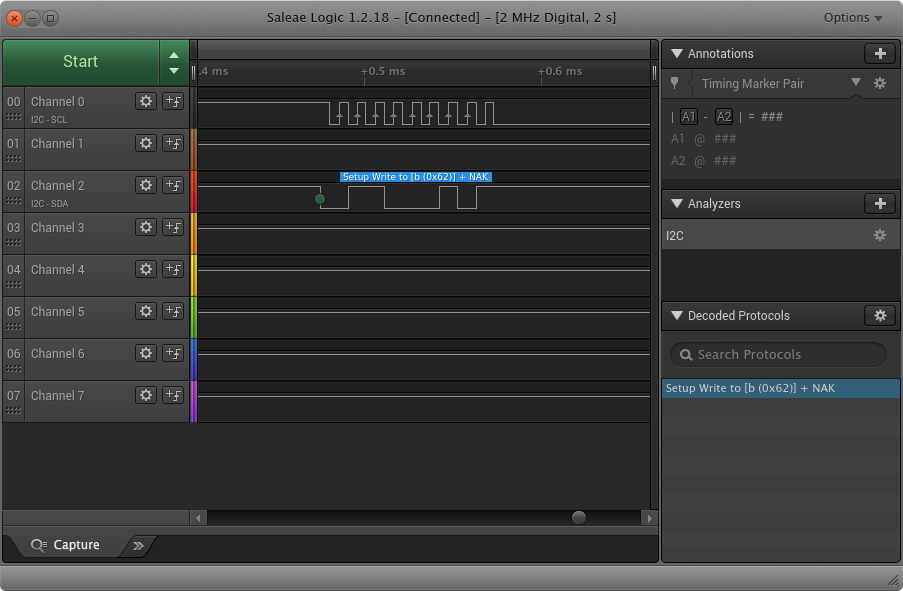
\includegraphics[height=0.22\textheight]{figures/v05/waveform-i2c-2.png}}
        \caption{I$^{2}$C port 2 test.}
        \label{fig:test-i2c-2}
    \end{center}
\end{figure}

%\begin{figure}[!ht]
%    \begin{center}
%        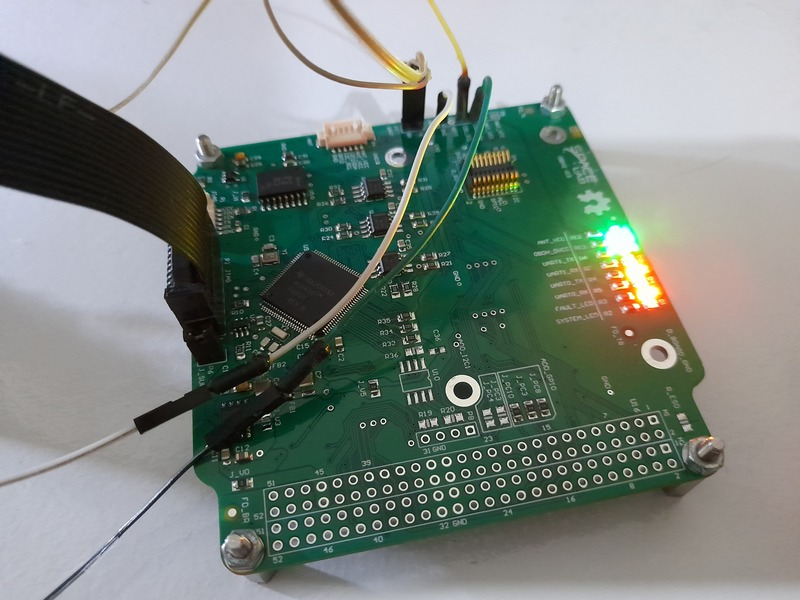
\includegraphics[width=0.7\columnwidth]{figures/v05/test-i2c-2.jpg}
%        \caption{Connections of the I2C port 2 test.}
%        \label{fig:test-i2c-2}
%    \end{center}
%\end{figure}
%
%\begin{figure}[!ht]
%    \begin{center}
%        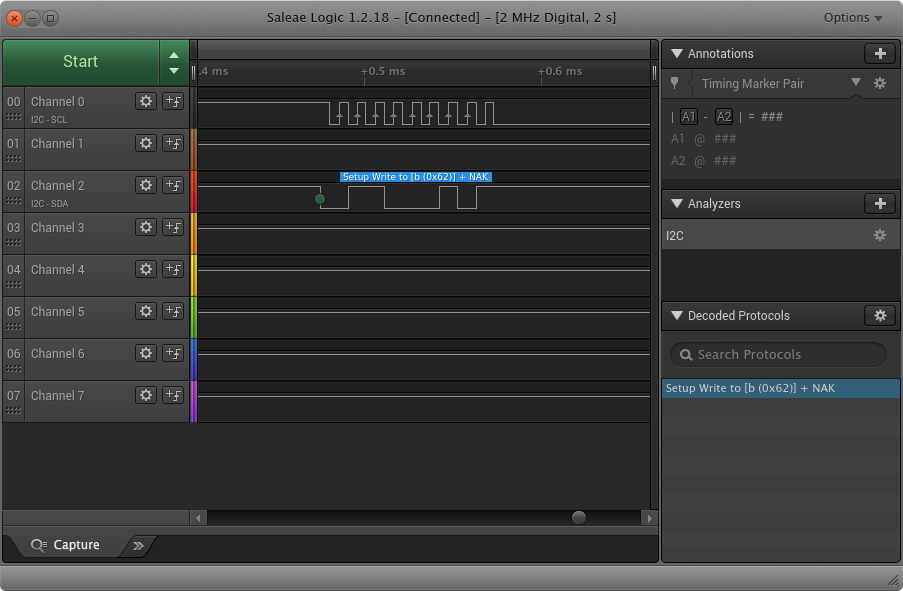
\includegraphics[width=\columnwidth]{figures/v05/waveform-i2c-2.png}
%        \caption{Waveform of the I2C port 2.}
%        \label{fig:waveform-i2c-2}
%    \end{center}
%\end{figure}

\section{Sensors}

\subsection{Input Voltage}

\begin{itemize}
    \item \textbf{Test description/Objective}: .
    \item \textbf{Material}:
        \begin{itemize}
            \item Code Composer Studio v9.3.0
            \item MSP-FET Flash Emulation Tool
            \item USB-UART converter
            \item Screen (Linux software)
        \end{itemize}
    \item \textbf{Results}: .
    \item \textbf{Conclusion:} .
\end{itemize}

\subsection{Input Current}

\begin{itemize}
    \item \textbf{Test description/Objective}: .
    \item \textbf{Material}:
        \begin{itemize}
            \item Code Composer Studio v9.3.0
            \item MSP-FET Flash Emulation Tool
            \item USB-UART converter
            \item Screen (Linux software)
        \end{itemize}
    \item \textbf{Results}: .
    \item \textbf{Conclusion:} .
\end{itemize}

\begin{figure}[!htb]
    \begin{center}
        \subfigure[Current sensing circuit.\label{fig:current-sensing-circuit-v05}]{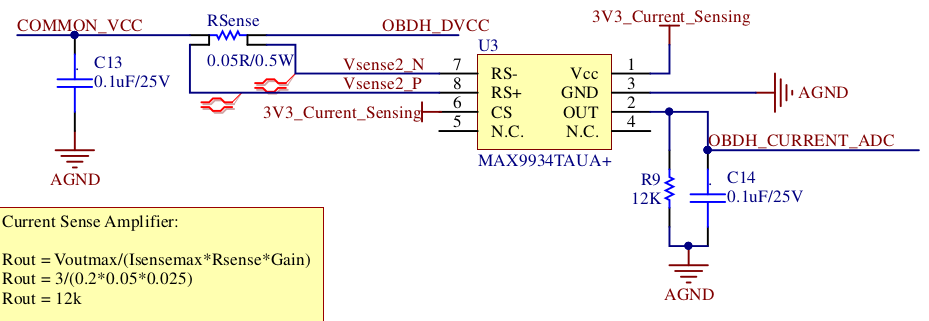
\includegraphics[width=0.8\textwidth]{figures/v05/current-sensor-circuit.png}}

        \subfigure[MAX9934 pinout.\label{fig:max9934-pinout}]{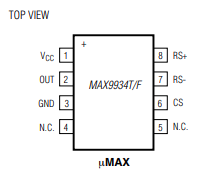
\includegraphics[width=0.4\textwidth]{figures/v05/max9934-top-view.png}}
        ~
        \subfigure[Current sensing layout (bottom layer).\label{fig:}]{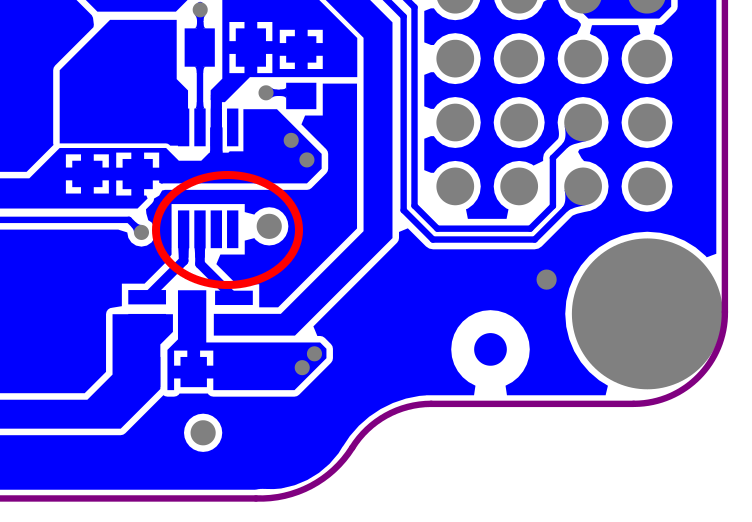
\includegraphics[width=0.4\textwidth]{figures/v05/current-sensor-layout.png}}
        \caption{.}
        \label{fig:current-sensing-error-v05}
    \end{center}
\end{figure}

\begin{figure}[!ht]
    \begin{center}
        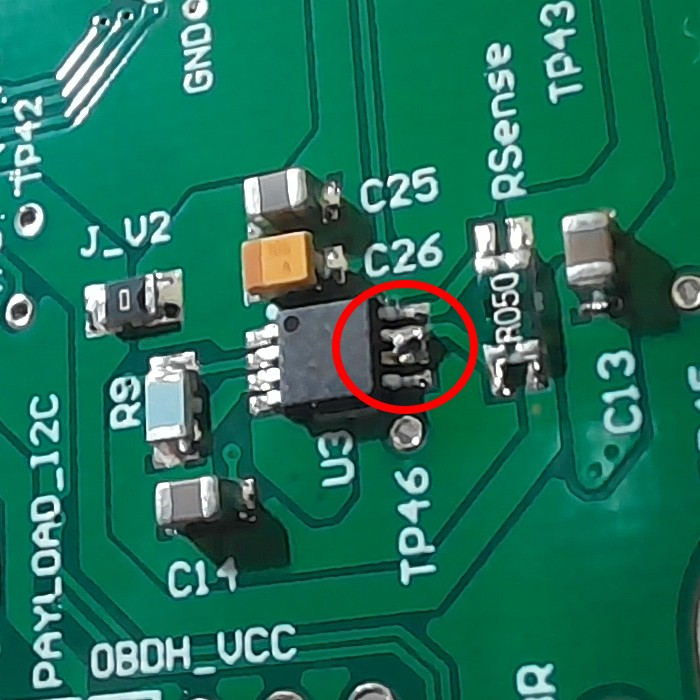
\includegraphics[width=0.6\columnwidth]{figures/v05/max9934-fix.jpg}
        \caption{Current sensor fix.}
        \label{fig:current-sensor-fix}
    \end{center}
\end{figure}

\begin{figure}[!ht]
    \begin{center}
        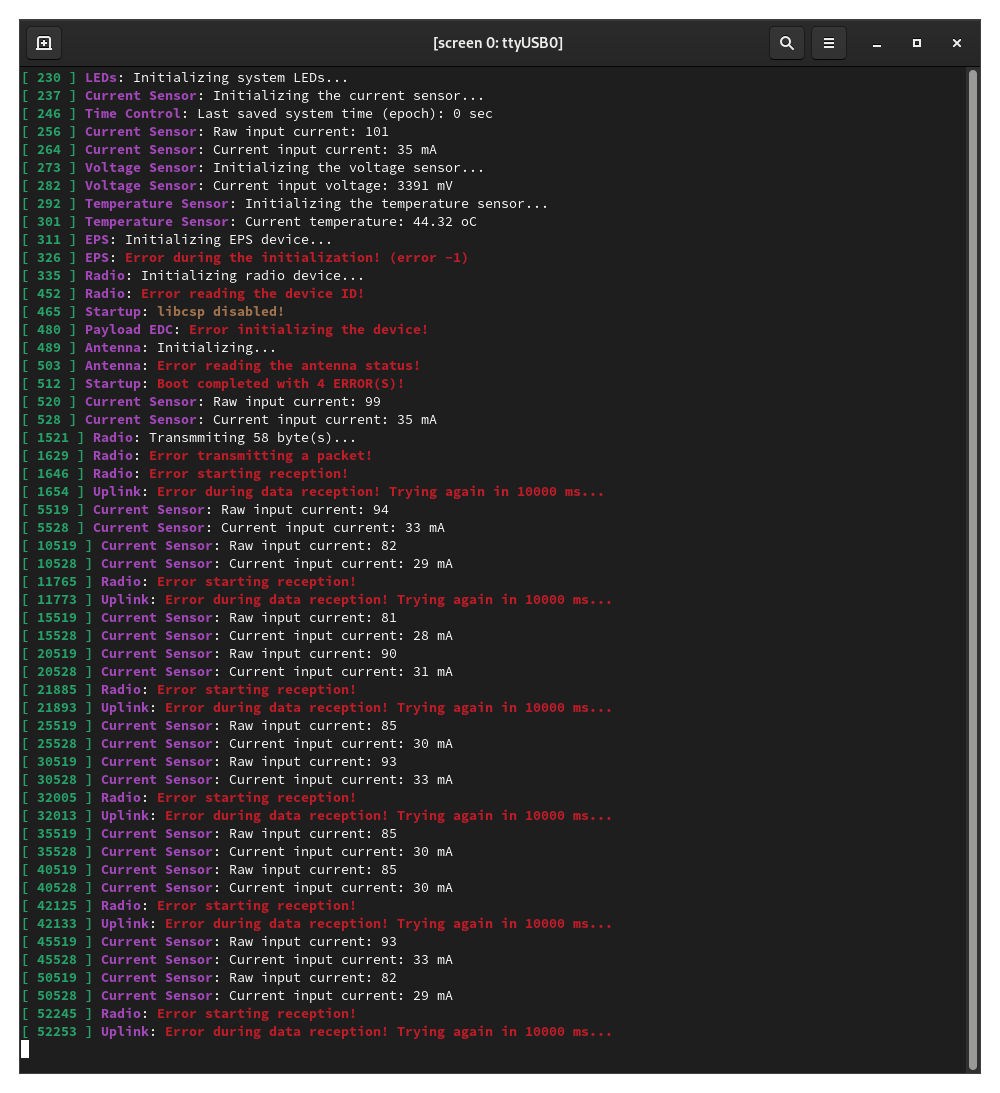
\includegraphics[width=0.7\columnwidth]{figures/v05/log-current-sensor.png}
        \caption{Log messages with the read values from the current sensor.}
        \label{fig:log-current-sensor}
    \end{center}
\end{figure}

\section{Peripherals}

\subsection{NOR Flash Memory}

\begin{itemize}
    \item \textbf{Test description/Objective}: Test the functionality of the NOR flash memory by verifying the device ID register of the IC.
    \item \textbf{Material}:
        \begin{itemize}
            \item Saleae Logic Analyzer (24 MHz, 8 channels)
            \item Saleae Logic software (v1.2.18)
            \item MSP-FET Flash Emulation Tool
        \end{itemize}
    \item \textbf{Results}: The results of this test can be seen in \autoref{fig:test-nor-memory}.
    \item \textbf{Conclusion:} No problems were identified on this test, as can be seen in \autoref{fig:waveform-spi-mem}, the device ID register was read as expected.
\end{itemize}

\begin{figure}[!htb]
    \begin{center}
        \subfigure[Connections of the NOR flash memory test.\label{fig:connections-nor-memory}]{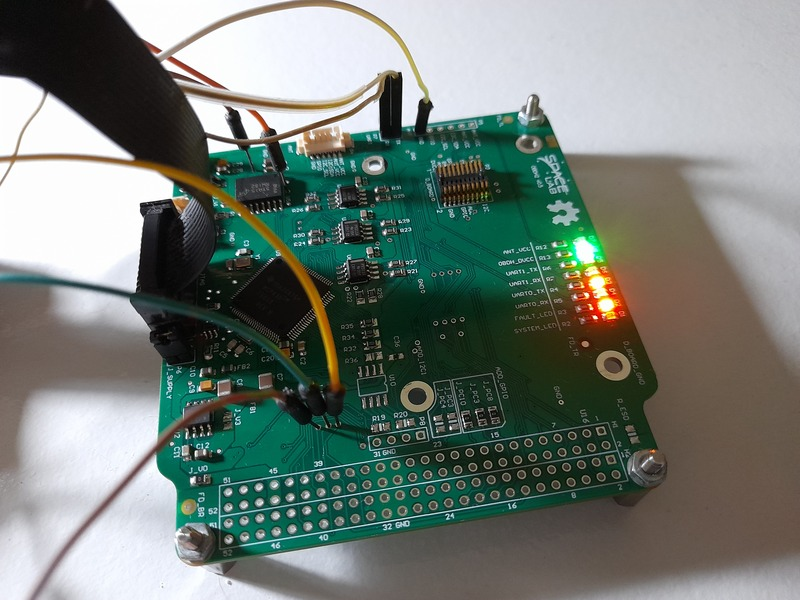
\includegraphics[height=0.22\textheight]{figures/v05/test-nor-memory.jpg}}
        ~
        \subfigure[Waveforms of the NOR memory SPI.\label{fig:waveform-spi-mem}]{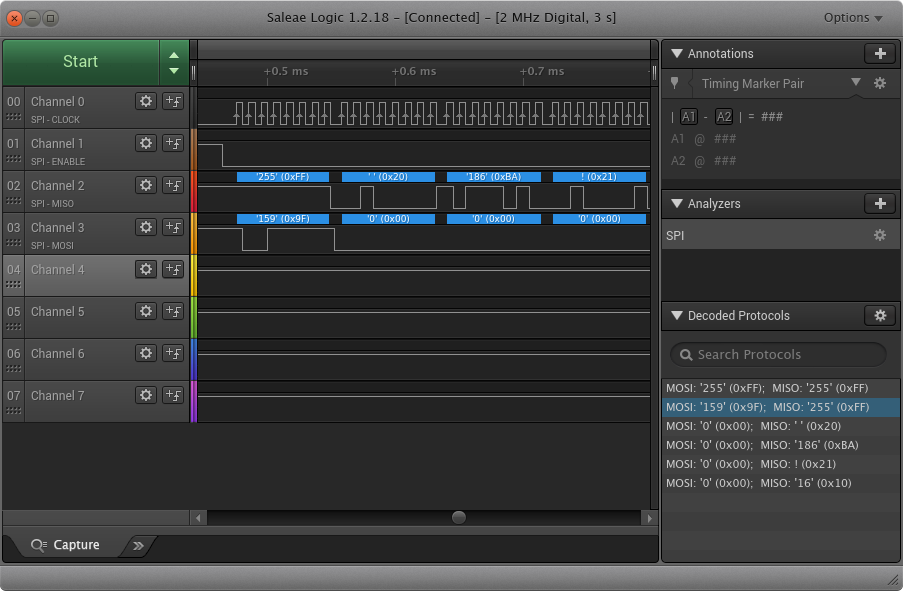
\includegraphics[height=0.22\textheight]{figures/v05/waveform-spi-mem.png}}
        \caption{NOR memory SPI test.}
        \label{fig:test-nor-memory}
    \end{center}
\end{figure}

%\begin{figure}[!ht]
%    \begin{center}
%        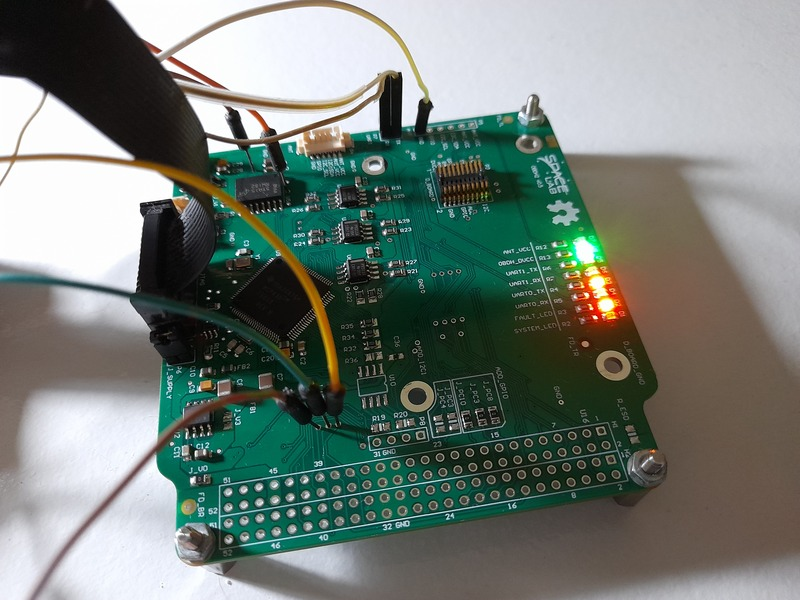
\includegraphics[width=0.7\columnwidth]{figures/v05/test-nor-memory.jpg}
%        \caption{Connections of the NOR flash memory test.}
%        \label{fig:test-nor-memory}
%    \end{center}
%\end{figure}
%
%\begin{figure}[!ht]
%    \begin{center}
%        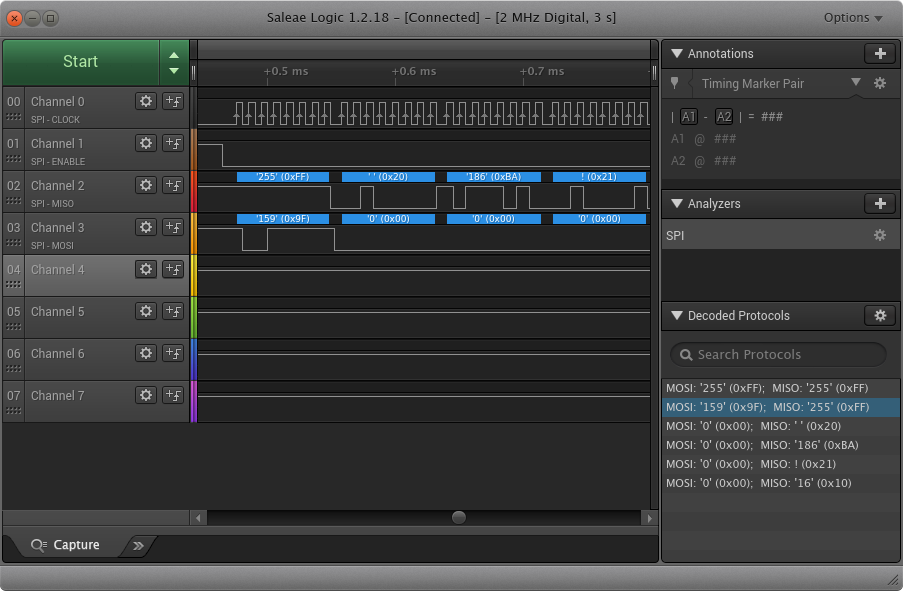
\includegraphics[width=\columnwidth]{figures/v05/waveform-spi-mem.png}
%        \caption{Waveform of the NOR memory SPI.}
%        \label{fig:waveform-spi-mem}
%    \end{center}
%\end{figure}

\section{Conclusion}

Excluding the current sensor issue, no major problems were identified during the executed tests. For the next fabrication round, the identified mistakes will be corrected.
